\documentclass{article}

\usepackage{graphicx} % Required for the inclusion of images
\usepackage{natbib} % Required to change bibliography style to APA
\usepackage{amsmath} % Required for some math elements 



\usepackage{amssymb}
\usepackage{amsmath}
\usepackage{float}

\usepackage{caption}

\usepackage{enumitem}
\usepackage{booktabs}

\usepackage{multirow}

\usepackage{amsmath}

\usepackage{subcaption}
\captionsetup{compatibility=false}

\floatstyle{plaintop}
\restylefloat{table}



\setlength\parindent{0pt} % Removes all indentation from paragraphs

\renewcommand{\labelenumi}{\alph{enumi}.} % Make numbering in the enumerate environment by letter rather than number (e.g. section 6)

%\usepackage{times} % Uncomment to use the Times New Roman font

%----------------------------------------------------------------------------------------
%	DOCUMENT INFORMATION
%----------------------------------------------------------------------------------------

\title{Biometrics \\ Laboratory Report} % Title

\author{Jakub \textsc{Ciecierski}} % Author name

\date{\today} % Date for the report

\begin{document}

\maketitle % Insert the title, author and date

\begin{center}
\begin{tabular}{l r}
Date Performed: & October 16, 2015 \\ % Date the experiment was performed
\end{tabular}

\vspace{60pt}

\includegraphics[width=80mm]{res/mini.PNG} \\
\end{center}

% If you wish to include an abstract, uncomment the lines below
% \begin{abstract}
% Abstract text
% \end{abstract}

\newpage

	\tableofcontents
	
\newpage


%----------------------------------------------------------------------------------------

\section{Objective}
The objective of the laboratory was to apply certain image processing methods.
This study was concerned with the following methods:
\begin{itemize}
	\item Threshold.
	\item Histogram Expansion.
	\item Brightness
\end{itemize}

In section~\ref{sec:methodology}, I will describe in details all the methods and their variations.

The experiments will be conducted in section~\ref{sec:experiment} where I compare and analyse different results for each algorithms.

I will finish with conclusions in section~\ref{sec:conclusions}

%----------------------------------------------------------------------------------------

\section{Methodology}
\label{sec:methodology}

%----------------------------------------------------------------------------------------
%----------------------------------------------------------------------------------------

\subsection{Threshold}
The first algorithm being described in Thresholding.
I assume that the input image is in gray scale, tresholding can be also applied to color images but for simplicity of the experiments I only worked with gray scale.
The algorithm is as follows:
\begin{enumerate}
	\item Choose constant $0 < T < 255$
	\item For each pixel in input image (gray scale)
	\begin{enumerate}
		\item If pixel intensity is lower than T
		then set value of that pixel to 0. \\
		Otherwise set it to 255.
	\end{enumerate}
\end{enumerate}

The most important part of thresholding is finding a proper value for the actual threshold $T$.
The big problem with this algorithm is that we only consider the pixel's intensities, not the relation between pixels.
Thus by setting improper constant value of $T$ might lead to loosing important information about the image.

During the laboratories, we did not try other methods of setting the threshold, but it is important to mention them.
We can use the adaptive thresholding such as:
\begin{itemize}
	\item Threshold value is the mean of neighbourhood area.
	
	\item  Threshold value is the weighted sum of neighbourhood values 					where weights are a gaussian window.		
\end{itemize}

Later during the experiment we shall test out results for different values of $T$.

%----------------------------------------------------------------------------------------
%----------------------------------------------------------------------------------------
\subsection{Histogram Expansion}
Also known as Histogram stretching or simply Normalization, this algorithm is a process of changing the range of pixel intensity values.

The new value of intensity of a pixel is changed as follows:
\begin{equation}
\label{eq:hist_exp}
 I_n = (I - min) * ((desiredMax - desiredMin) / (max - min)) + desiredMin
\end{equation}

where $max$, $min$ is the maximum and minimum intensities in the input image respectively.
$desiredMax$, $desiredMin$ is the desired range which we want to stretch the histogram to. In our case these variables take the following values:\\
$desiredMax = 255$, $desiredMin = 0$.

During the laboratories we conducted histogram expansion with two variations on finding maximum and minimum intensities.

\begin{itemize}
	\item The maximum and minimum were computed by taking the average of three channels for each pixel. Let us denote this variation by $AVG\_MIN/MAX$
	\item The maximum and minimum were computed for each channel individually, thus giving us three maximums and three minimums - each for every channel. This one will be denoted $ALL\_MIN/MAX$
\end{itemize}

In either case, the equation~\ref{eq:hist_exp} was applied to each channel individually.

The potential problem with $AVG\_MIN/MAX$ algorithm might occur when a certain pixel intensity has a much higher value for one channel than the others. In such case this channel might be considered an outlier.

%----------------------------------------------------------------------------------------
%----------------------------------------------------------------------------------------
\subsection{Brightness}
The last algorithm we consider is the simplest.

\begin{enumerate}
	\item Choose a constant brightness $B$
	\item For each pixel of the input image increase the value of pixel's channel by brightness $B$
\end{enumerate}

It is worth mentioning that when increasing values of pixel's intensity we must be careful with upper bound - do not overflow the maximum value of one byte - namely 255.

%----------------------------------------------------------------------------------------

\section{Experiment}
\label{sec:experiment}

Figure~\ref{fig:source_img} presents the images that will be used in our experiments. First we will show how gray scale image behaves for thresholding with different threshold values. Then both original and grayscale images will be subjected to histogram expansion. Lastly we observe results for brightness filter.


\begin{figure}[H]
\centering

\begin{subfigure}{.5\textwidth}
  \centering
  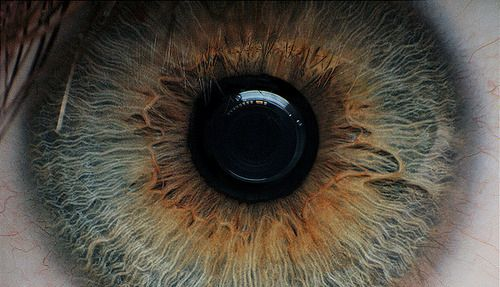
\includegraphics[width=0.9\linewidth]{res/index.jpg}
  \caption{Original image}
  \label{fig:original_img}
\end{subfigure}%
\begin{subfigure}{.5\textwidth}
  \centering
  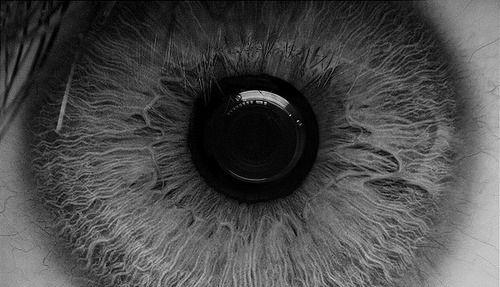
\includegraphics[width=0.9\linewidth]{res/grayscale.jpg}
  \caption{Grayscale image}
  \label{fig:gray_img}
\end{subfigure}

\caption{The original and grayscale pictures used in experiments}
\label{fig:source_img}
\end{figure}






%----------------------------------------------------------------------------------------
%----------------------------------------------------------------------------------------
\subsection{Threshold}
Figure~\ref{fig:threshold} presents results for thresholding a grayscale image for different values of threshold. It was mentioned in the methodology section that choosing a proper threshold is important or else the information about an image can be lost. This assumption is verified with our results. Looking at the threshold value of 25 we can see that too many pixels became white. On the other hand in the threshold equal to 150 we observe the opposite - most of the pixels are black. In both cases we lose information. The best out of the four tested thresholds seems to be the value 50.



% THRESHOLD
\begin{figure}[H]
\centering

\begin{subfigure}[b]{0.5\linewidth}
\centering
  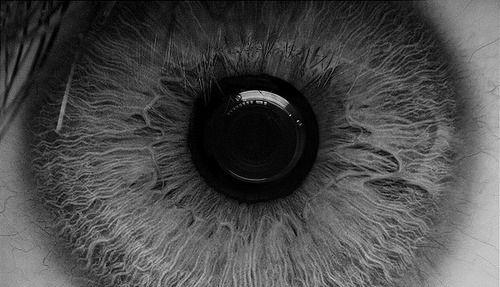
\includegraphics[width=0.9\linewidth]{res/grayscale.jpg}
  \caption{The grayscale image}
   \label{fig:tresh_gray}
\end{subfigure}%

\begin{subfigure}[b]{0.5\linewidth}
\centering
  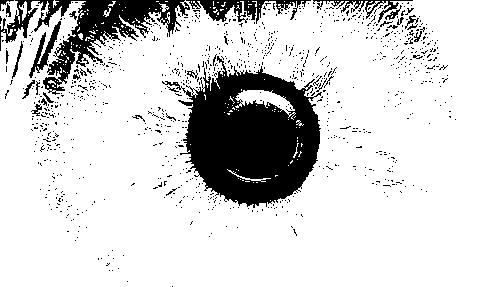
\includegraphics[width=0.9\linewidth]{res/tresh25.jpg}
  \caption{Threshold 25}
   \label{fig:tresh_25}
\end{subfigure}%
\begin{subfigure}[b]{0.5\linewidth}
\centering
  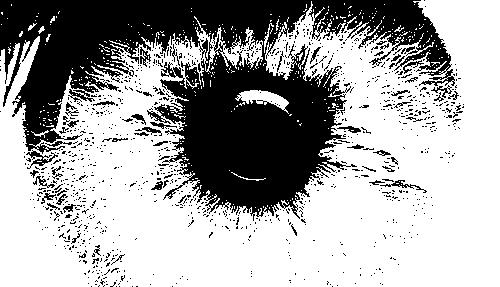
\includegraphics[width=0.9\linewidth]{res/tresh50.jpg}
  \caption{Threshold 50}
   \label{fig:original}
\end{subfigure}%

\begin{subfigure}[b]{0.5\linewidth}
\centering
  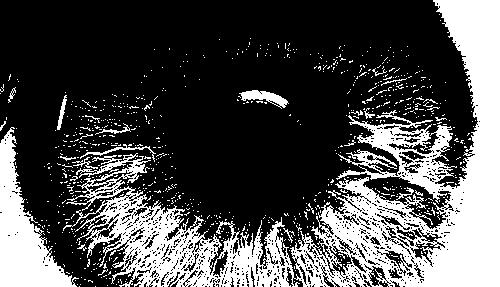
\includegraphics[width=0.9\linewidth]{res/tresh100.jpg}
  \caption{Threshold 100}
   \label{fig:original}
\end{subfigure}%
\begin{subfigure}[b]{0.5\linewidth}
\centering
  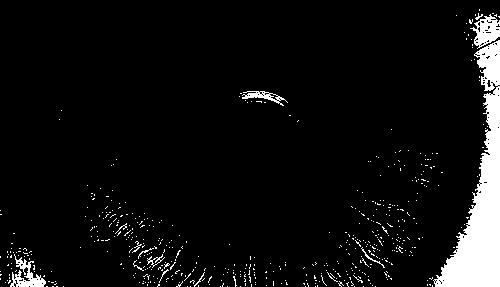
\includegraphics[width=0.9\linewidth]{res/tresh150.jpg}
  \caption{Threshold 150}
   \label{fig:original}
\end{subfigure}%


  
  \caption{The grayscale image and thresholded images for different threshold values.}
  \vspace{-12pt}
  \label{fig:threshold}

\end{figure}


%----------------------------------------------------------------------------------------
%----------------------------------------------------------------------------------------
\subsection{Histogram Expansion}
Let us start of by showing the results of stretching a histogram of a grayscale image. Figure~\ref{fig:histogram_gray} is the point of interest in this case. It should not be a surprise that figures~\ref{fig:hist_gray_all} and~\ref{fig:hist_gray_avg} are exactly the same. Recall that in grayscale images, pixels have the same values for each channel. Let us carefully observe between the grayscale image in~\ref{fig:hist_gray_org} and the other two.
We can clearly see improvement in quality in the normalized images. The nearly white pixels became cleaner - or simply they became even more white. The same happened for black pixels. Overall the image becomes more sharp and detailed.


% HISTOGRAM GRAY
\begin{figure}[H]
\centering

\begin{subfigure}[b]{0.5\linewidth}
\centering
  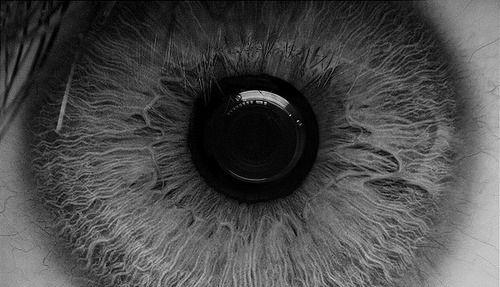
\includegraphics[width=0.9\linewidth]{res/grayscale.jpg}
  \caption{The grayscale image}
   \label{fig:hist_gray_org}
\end{subfigure}%

\begin{subfigure}[b]{0.5\linewidth}
\centering
  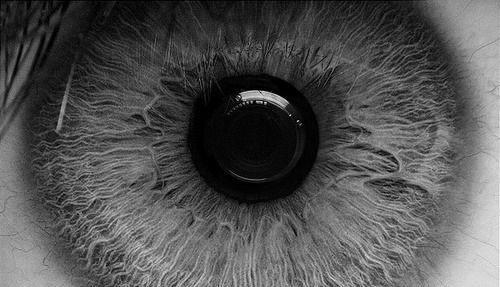
\includegraphics[width=0.9\linewidth]{res/gray_hist_all.jpg}
  \caption{Histogram Expansion \\ ALL\_MIN/MAX}
   \label{fig:hist_gray_all}
\end{subfigure}%
\begin{subfigure}[b]{0.5\linewidth}
\centering
  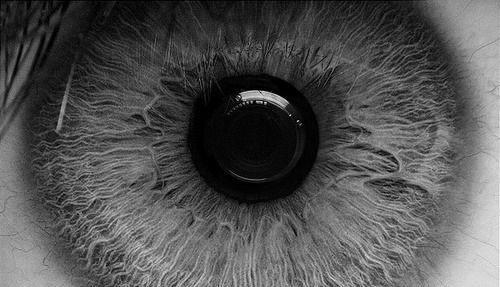
\includegraphics[width=0.9\linewidth]{res/gray_hist_avg.jpg}
  \caption{Histogram Expansion \\ AVG\_MIN/MAX}
   \label{fig:hist_gray_avg}
\end{subfigure}%


  \caption{The grayscale image and grayscale images after normalization with different methods of finding maximum and minimum pixel intensities.}
\vspace{-12pt}
  \label{fig:histogram_gray}
\end{figure}




The results for normalization of color image is presented in figure~\ref{fig:histogram_clr}.
Here we can see that that the normalization in which maximum and minimum was calculated separately (figure~\ref{fig:hist_clr_all}) for each channel yields slightly different results than the one with computed the average intensities (figure~\ref{fig:hist_clr_avg}).
The former one appears to be more detailed than the latter one.


% HISTOGRAM COLOR
\begin{figure}[H]
\centering

\begin{subfigure}[b]{0.5\linewidth}
\centering
  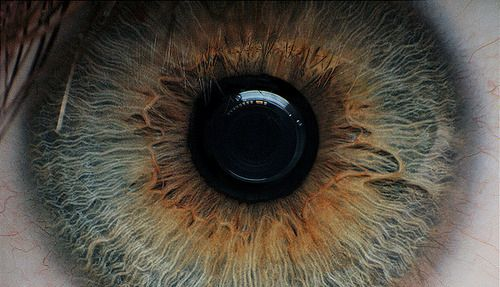
\includegraphics[width=0.9\linewidth]{res/index.jpg}
  \caption{The original image}
   \label{fig:hist_clr_org}
\end{subfigure}%

\begin{subfigure}[b]{0.5\linewidth}
\centering
  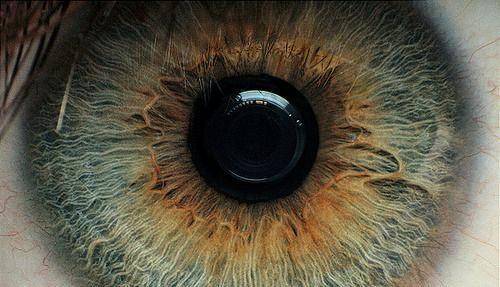
\includegraphics[width=0.9\linewidth]{res/hist_all.jpg}
  \caption{Histogram Expansion \\ ALL\_MIN/MAX}
   \label{fig:hist_clr_all}
\end{subfigure}%
\begin{subfigure}[b]{0.5\linewidth}
\centering
  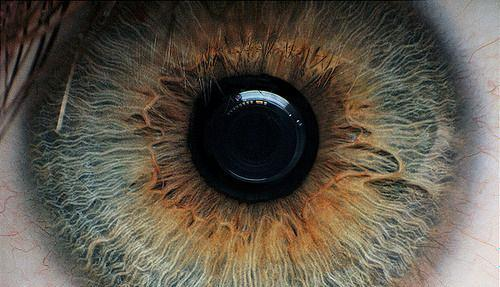
\includegraphics[width=0.9\linewidth]{res/hist_avg.jpg}
  \caption{Histogram Expansion \\ AVG\_MIN/MAX}
   \label{fig:hist_clr_avg}
\end{subfigure}%




  \caption{The original image and images after normalization with different methods of finding maximum and minimum pixel intensities.}
  
\vspace{-12pt}
  \label{fig:histogram_clr}
\end{figure}













%----------------------------------------------------------------------------------------
%----------------------------------------------------------------------------------------
\subsection{Brightness}

Lastly we consider the process of brightening an image. As before, the original image was subjected to filtering for different values of brightness. This is presented in the figure~\ref{fig:brightness}.
With bigger brightness, the pixels become more white. Very big value can make the image look unattractive.




% BRIGHTNESS
\begin{figure}[H]
\centering

\begin{subfigure}[b]{0.5\linewidth}
\centering
  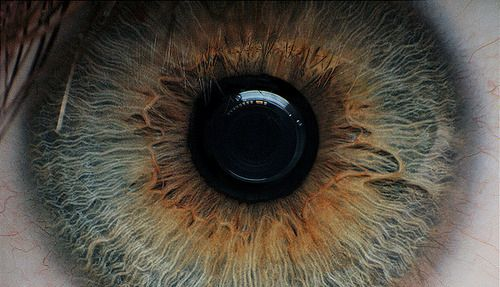
\includegraphics[width=0.9\linewidth]{res/index.jpg}
  \caption{The original image}
   \label{fig:bright_org}
\end{subfigure}%

\begin{subfigure}[b]{0.5\linewidth}
\centering
  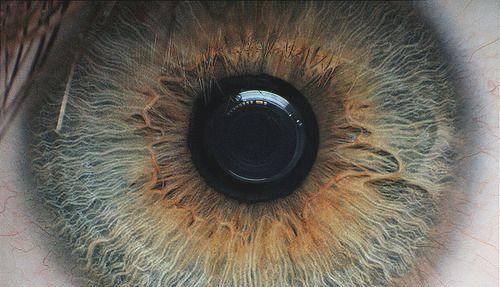
\includegraphics[width=0.9\linewidth]{res/bright25.jpg}
  \caption{Brightness 25}
   \label{fig:bright_25}
\end{subfigure}%
\begin{subfigure}[b]{0.5\linewidth}
\centering
  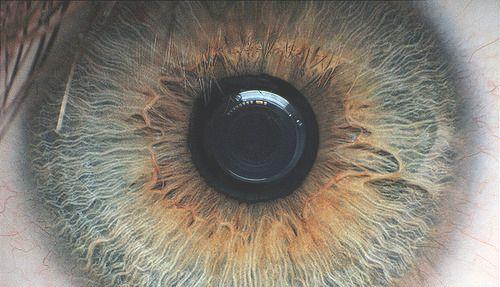
\includegraphics[width=0.9\linewidth]{res/bright50.jpg}
  \caption{Brightness 50}
   \label{fig:bright_50}
\end{subfigure}%

\begin{subfigure}[b]{0.5\linewidth}
\centering
  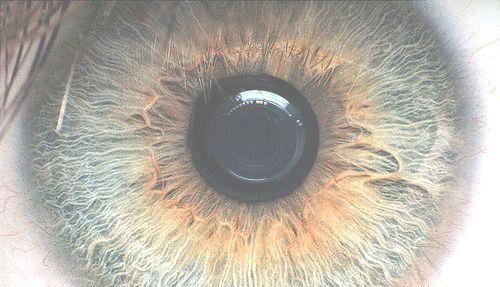
\includegraphics[width=0.9\linewidth]{res/bright100.jpg}
  \caption{Brightness 100}
   \label{fig:bright_100}
\end{subfigure}%
\begin{subfigure}[b]{0.5\linewidth}
\centering
  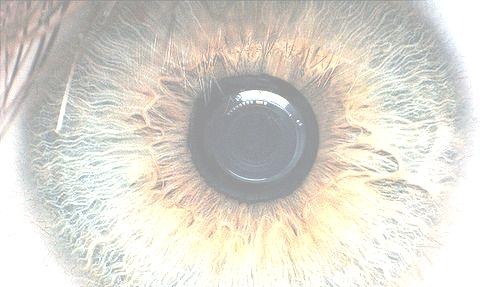
\includegraphics[width=0.9\linewidth]{res/bright150.jpg}
  \caption{Brightness 150}
   \label{fig:bright_150}
\end{subfigure}%



  \caption{The original image and images with different brightness values.}
\vspace{-12pt}
  \label{fig:brightness}
\end{figure}








%----------------------------------------------------------------------------------------

\section{Conclusions}
\label{sec:conclusions}

In our laboratories we tested three different image processing algorithms, the thresholding, histogram expansion and brightness.

We showed that choosing a proper threshold is important as not doing so might lead to information lose.

We applied histogram expansion for two different variations. Choosing the maximum and minimum individually for each channel showed better results.
%----------------------------------------------------------------------------------------
%	BIBLIOGRAPHY
%----------------------------------------------------------------------------------------

\bibliographystyle{apalike}

\bibliography{sample}

%----------------------------------------------------------------------------------------


\end{document}